\begin{figure*}[htbp]
\centering
\vspace{-2mm}
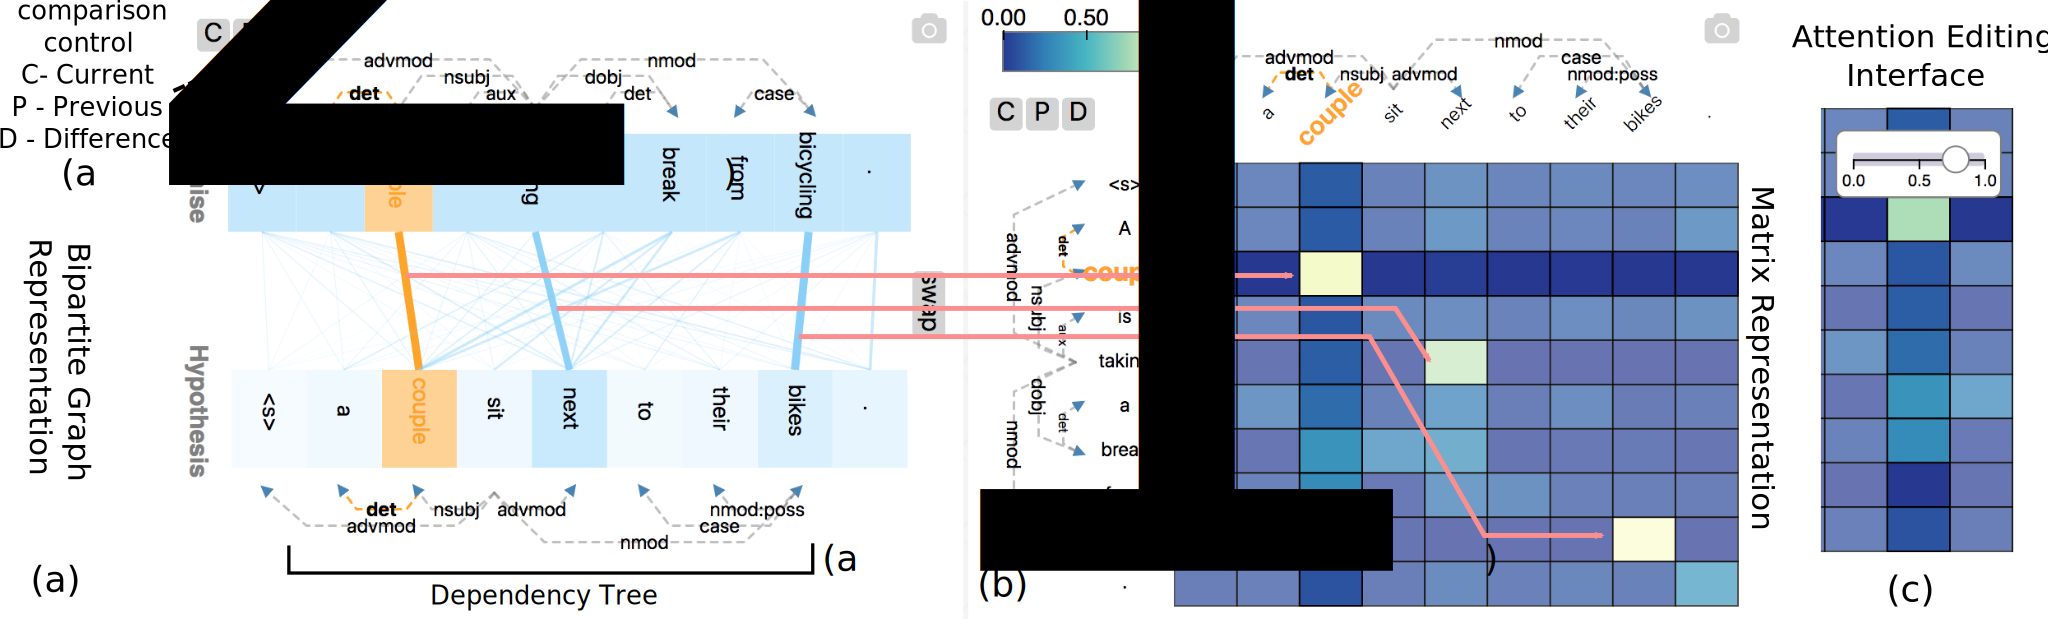
\includegraphics[width=1.0\linewidth]{attentionView}
\vspace{-6mm}
\caption{
Attention visualization. In the graph attention view (a), a bipartite graph encoding is adopted, in which the edge thickness corresponds to the attention value. In the matrix attention view (b), the entries of $i^{th}$ row represent the probabilities of words in hypotheses align to the $i^{th}$ word in the premise.
The user can alter the attention values via the pop-up interface illustrated in (c).
We overlay the dependency tree ($a_1$) grammar structure to highlight important words and simplify complex sentence to reduce clutter (d-e).
In (f), we show the difference between two attention matrix (the comparison feature is controlled by the buttons in the top left of all attention plots ($a_2$) ).
}
\label{fig:attentionVis}
\vspace{-4mm}
\end{figure*}

\subsection{Sentence View}
\label{sec:sentence}
% Once an exploration cycle started, the experts need to examine the premise and hypothesis sentence the current example.
As illustrated in Fig.~\ref{fig:teaser}(B), the sentence view shows the premise and hypothesis sentence.
%
To facilitate the analysis task (\textbf{T1}), we employ an automate sentence perturbation scheme that replaces \emph{nouns} and \emph{verbs} by their synonyms in the wordNet~\cite{Miller1995} (the standard lexical database for NLP applications).
%
When the perturbation is applied to either of the sentences, the replaced words are highlighted in blue to signal the modification made to the original sentence.

% \begin{figure}[htbp]
% \centering
% \vspace{-2mm}
%  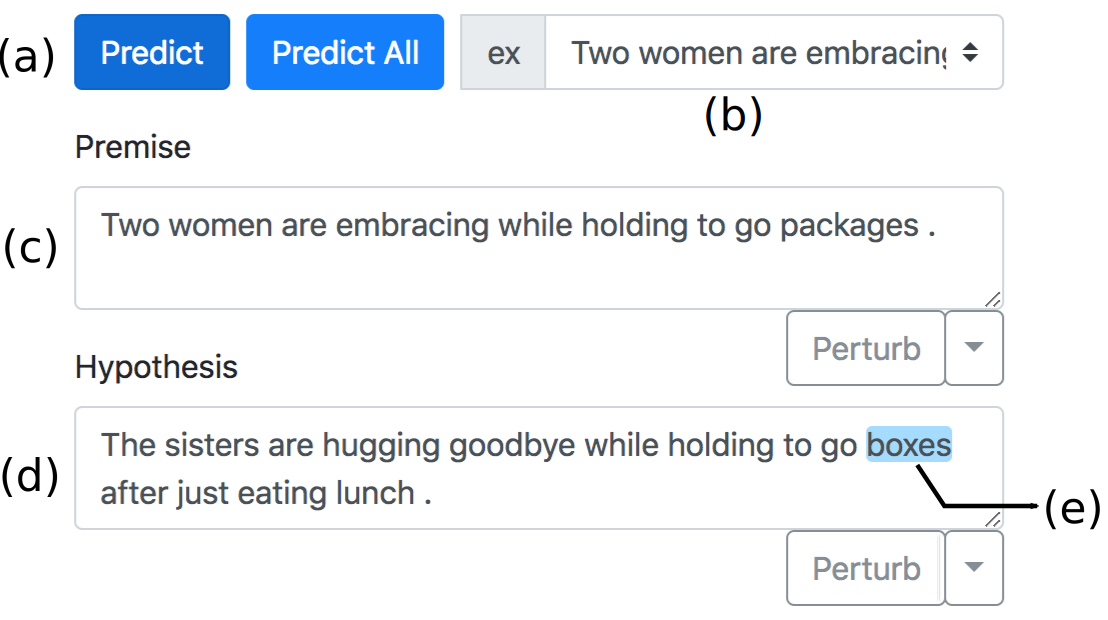
\includegraphics[width=0.9\linewidth]{sentenceView}
%  \vspace{-2mm}
%  \caption{
%  Sentence view shows the premise (c) and the hypothesis (d) sentence pair. The word that replaces the word in the original text is highlighted in blue (e).
%  The \emph{Predict} and \emph{Predict All} controls (a) correspond to predicting the currently displayed sentence pairs and predicting all combinations of perturbed premise and hypothesis, respectively.
%  Previous explored original sentence are stored in the dropdown list (d) that allow the user to revisit previous examined sentence.
% }
% \label{fig:sentenceView}
% \end{figure}


At the top left of the view, the two controls \emph{Predict} and \emph{Predict All} correspond to predicting the currently displayed sentence pairs and predict all combinations of perturbed premises and hypotheses, respectively.
%
To avoid the situation where both sentences are perturbed, we ensure only one perturbation per sentence pair (i.e., we use the original premise if the hypothesis is perturbed, or use the original hypothesis if the premise is perturbed).
%%% sentence perturbation %%%%
The previously explored original sentences are stored in the dropdown list (left of the buttons) that allow the user to revisit examined examples.
Also, the user can type any sentences or modified existing text in the sentence display areas to accommodate user-defined input.



%\begin{itemize}
%\item Examine perturbed pair
%\item See which word is perturbed in a sentence
%\item Add to existing example collection
%\end{itemize}
